\documentclass{article}
\usepackage[utf8]{inputenc}
\usepackage{graphicx}
\usepackage{epstopdf}
\usepackage{caption}
\usepackage{subcaption}
\usepackage{multirow}
\usepackage{hyperref}
\usepackage{url}
\usepackage{seqsplit}
\hypersetup{pdfstartview={FitH null null null}}
\usepackage{amssymb,amsmath}
\usepackage{amsthm}
\usepackage{empheq}
\usepackage{algorithm,algpseudocode}
\usepackage[margin=1.5in]{geometry}
\usepackage{listings}
\usepackage{program}
\lstset{language=Python} 

\usepackage{listings}
\usepackage{color} %red, green, blue, yellow, cyan, magenta, black, white
\definecolor{mygreen}{RGB}{28,172,0} % color values Red, Green, Blue
\definecolor{mylilas}{RGB}{170,55,241}


\title{Ab-initio modeling using a fragment matching and energy functions}
\author{Caiwei Wang, Xiaokai Qian, Sean Lander, Haipei Fan, Puneet Gaddam, Brett Koonce\\University of Missouri - Columbia}

\date{March 10, 2013}

\algloopdefx{NoEndIf}[1]{\textbf{If} #1 \textbf{then}}

\begin{document}

\maketitle

\section{Abstract}
This project is to develop a simple prototype of fragment assembly template-free modeling system. First, we convert PDB into residue-torsion pairs and use sliding window along to get lists for building fragment database created by Rosetta. Next, we can randomly select from list of matches. After initialization, we use simulated annealing to judge if the fragment’s neighbor can be accepted according to consensus scoring. Finally, we can get millions of decoys that are scored and sorted for evaluation. Ultimately, we create a movie of the top-scoring protein.

\section{Introduction}

Template free modeling is an important technique in modern bioinformatics since not all proteins have templates. First, we begin with PDB sequences converting into torsion angles using rama/lipa. By sliding window algorithm, we can get millions of fragments to construct the database. Then for each segment do a query for a complete match in the database.\\\\
We use simulated annealing to score, when the current solution’s neighbor is better, accepted. If not, we select it with a probability based on the current temperature. We modified consensus scoring for model acceptance. If the score improves for 2/3 through the scoring techniques D-fire energy function, accepted. Otherwise, do normalization and sum to be accepted upon temperature based probability.\\\\
For our project, we implemented basic homology modeling in python 3.3, using a number of external tools like D-fire, Rosetta, TM-score presenting a final visualized model.


\subsection{Pipeline}

\begin{figure}[H]
\begin{center}
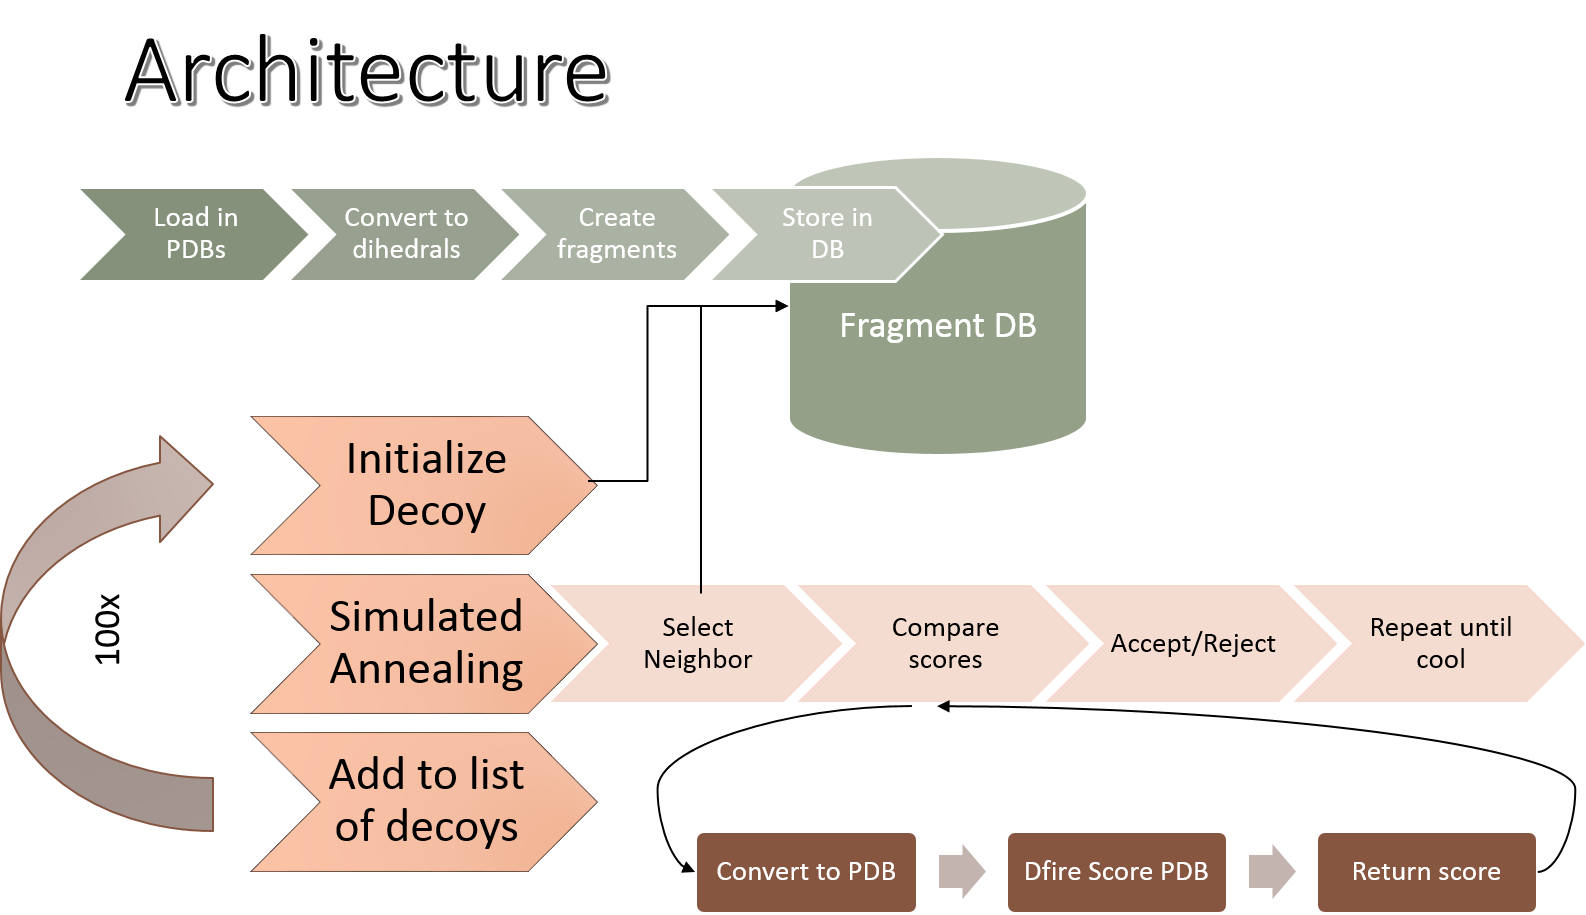
\includegraphics[width=\textwidth]{pipeline}
\caption{An overview of the TFPy pipeline}
\label{Fig:blosum}
\end{center}
\end{figure}

In order to more easily assemble our workflow we break it into a simple pipeline. Doing this allows for quick iteration on multiple fronts without the fear of breaking the model as a whole.

\begin{enumerate}

\item The first task involves building robust and well-indexed fragment databases for the three and nine length sequences. Once this is complete we are free to iterate over the simulated annealing algorithm itself.

\item Once the databases are built we create the tools necessary to initialize the candidate, choose its neighbor and score the neighbor, all of which are independent of the simulated annealing algorithm itself.

\item Initialization is less important in simulated annealing than most due to its stochastic nature, so a close approximation using fragments from the database are sufficient to build starting point.

\item Neighbor selection is more important, and fragment selection is a key component separated from the core code, as is described in our section on neighbor using Blosum62.

\item Scoring features in a similar manner, as the neighbor must be converted to a PDB file, scored with an external system, and then have its score returned and compared. In our current model D-fire energy is used to score the model.

\item Finally, multiple cooling solutions may be used, so allowing the user a choice using functional methods are preferred. We currently provide both linear and inverse-sigmoid cooling functions, with a temperature ranging from 2500 to 0 over 1000 iterations.\\

\end{steps}


Creating a system in this way leads to easy parallelization, as each decoy can be generated independent of the others. This allows for rapid decoy creation and comparison with no human component necessary beyond initial input.


\section{Target goal}

\subsection{CASP}

\section{Fragment database}

First, we selected a set of 17,000 PDB database with sequence lengths of 100-150 residues.  Then, for each PDB file, we split it into a collection of (residue, phi angle, psi angle) inputs.  We discard the first and last residue, since they only have one valid angle.  Next, we go through each PDB file sequentially for each three residues:
\begin{program}

  \FOR i:=1 \TO (length(PDB)-1)-3 \STEP 1 \DO
	a := PDB[i], b:= PDB[i+1], c:= PDB[i+2]
     	addToFragmentTrimersDatabase(a, phi_a, psi_a, b, phi_b, psi_b, c, phi_c, psi_c)\\\\
\END
\end{program}

Then, we repeat the process for each nine residues:

\begin{program}
  \FOR i:=1 \TO (length(PDB)-1)-9 \STEP 1 \DO
	a := PDB[i], b:= PDB[i+1], c:= PDB[i+2],  \dotso
	addToFragmentNinemersDatabase(a, phi_a, psi_a, b, phi_b, psi_b, c, phi_c, psi_c, \dotso)\\\\
\END
\end{program}

Finally, we create an index for each sequence in our databases, in order to speed up future lookups.  This produces a database of approximately 1.7 million indexes of a reasonable size (Trimer: ~150MB, Ninemer: ~500MB) which can be searched very quickly.

\section{Simulated annealing}



After building fragments database, we are going to build a model for our target with the database. The algorithm we use in the project is Simulated Annealing. SA is a generic probabilistic metaheuristic for the global optimization problem of locating a good approximation to the global optimum of a given function in a large search space. It is often used when the search space is discrete. For our project, Simulated Annealing algorithm is quite efficient. Rather than hill climbing, SA can allow a bad fragment replacement in high temperature, which may lead to a better overall model structure. \\\\
In each cycle, SA grabs the current solution’s neighbor. If the neighbor’s score is better, use
the neighbor as the current solution. If it’s not, select it with a probability based on the current temperature.\\\\
     Also cool schedule is an important factor in the SA algorithm. A good cool schedule can efficiently and quickly help us find the optimal solution. In our project, we adopted the sigmoid function. Of course, we made modification on the function to make it fit our project. So the final cool schedule is either sigmoid or linear:\\\\
\begin{equation*}
      T_s(k) =  -5000/(1+ exp(-k/200))+5000
    \end{equation*}
\begin{equation*}
      T_l(k) =  (-2500/1000)*k + 2500
    \end{equation*}

. We believe allowing a “bad” fragment replacement can make great contributions to the final models in the beginning. The cool schedule will stay in high temperature for a long time to make it happen. Besides, temperature will stays cold for a period in the end because we have already built a quite “good” structure for majority of fragments and we want keep it “good”. By this function, we can optimize our search and help us find good structures for targets.


\section{Simulated Annealing psuedocode}
\begin{figure}[H]
\begin{center}
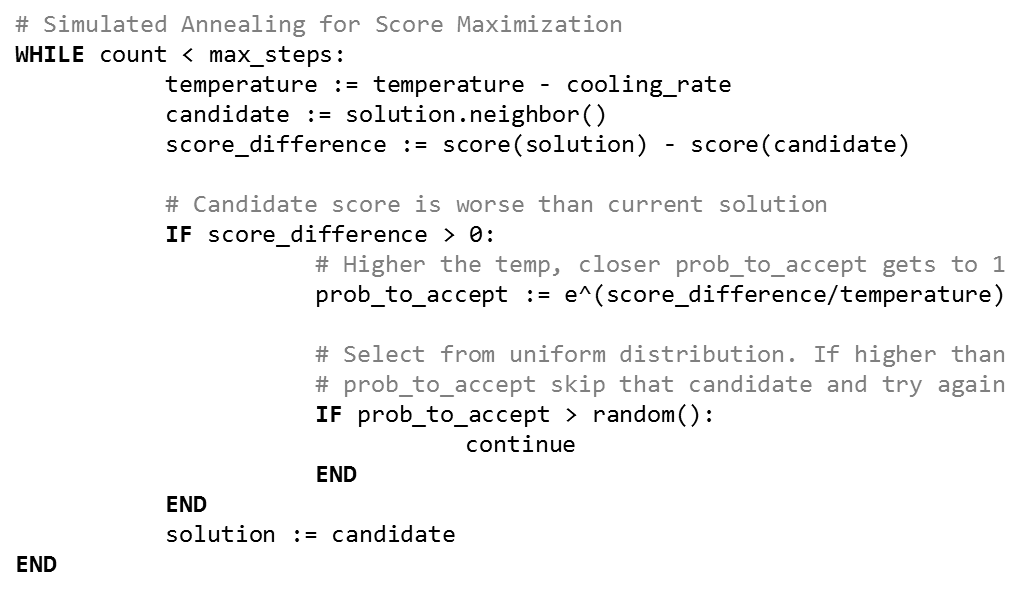
\includegraphics[width=\textwidth]{sa}
\label{Fig:blosum}
\end{center}
\end{figure}

\subsection{d-DFIRE score}

(need a section about dDFIRE

\subsection{BLOSUM62 selection}

Neighbor selection is an important part of greedy and semi-greedy algorithms, as changes which are too large can disrupt the process of finding global minima and maxima. In order to generate neighbors which are close to the current sequence we use a two-fold approach: find a complete match; if a match is not found, find a match for a very similar sequence. The first approach is easy to understand, but the second requires domain knowledge of amino acids, as some acids are more similar than others.\\

The Blosum62 matrix is a pair-wise "distance" matrix of sorts which can be used to determine the similarity of two amino acids. This matrix is commonly used to determine sequence similarity for alignment purposes, but can also be used as a generative model. By finding similar amino acids to those in the current fragment sequence, we can generate multiple sequences which are very similar in terms of "distance," allowing us to expand our search criteria on limited databases.

\newpage
\section{Visualization}

After we obtain our final target PDB file, we use Jmol to visualize it. At the same time, we also visualize the native one to compare it with our prediction.  The left one is a target structure we generated (T0644), while right one is the native structure.

\begin{figure}
\centering
\begin{minipage}{.5\textwidth}
  \centering
  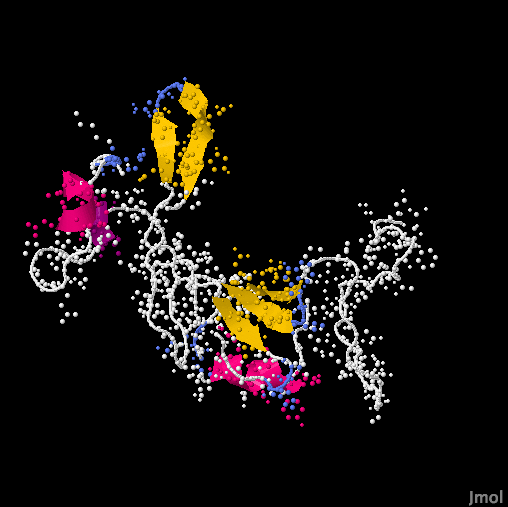
\includegraphics[width=.9\linewidth]{target_group_v2}
  \captionof{figure}{Target structure}
  \label{fig:test1}
\end{minipage}%
\begin{minipage}{.5\textwidth}
  \centering
  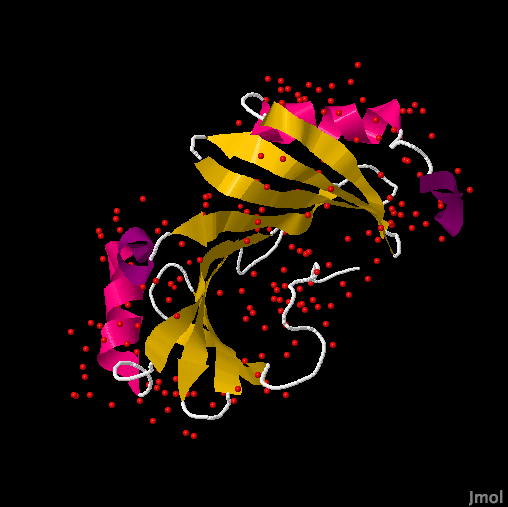
\includegraphics[width=.9\linewidth]{target_native}
  \captionof{figure}{Native structure}
  \label{fig:test2}
\end{minipage}
\end{figure}

\section{Results/statistics}



\subsection{Scores}
\begin{center}
    \begin{tabular}{ | l | l | l | p{2cm} |}
    \hline

    \hline
    \end{tabular}
\end{center}

\subsection{Future improvements}



\section{Citations}

We thank the following tools and papers: \\\\




\end{document}


\end{document}
